%\documentstyle[epsf,twocolumn]{jarticle}       %LaTeX2e仕様
%\documentclass[twocolumn]{jarticle}     %pLaTeX2e仕様(platex.exeの場合)
\documentclass[onecolumn]{ujarticle}   %pLaTeX2e仕様(uplatex.exeの場合)
%%%%%%%%%%%%%%%%%%%%%%%%%%%%%%%%%%%%%%%%%%%%%%%%%%%%%%%%%%%%%%
%%
%%  基本バージョン
%%
%%%%%%%%%%%%%%%%%%%%%%%%%%%%%%%%%%%%%%%%%%%%%%%%%%%%%%%%%%%%%%%%
\setlength{\topmargin}{-45pt}
%\setlength{\oddsidemargin}{0cm}
\setlength{\oddsidemargin}{-7.5mm}
%\setlength{\evensidemargin}{0cm}
\setlength{\textheight}{24.1cm}
%setlength{\textheight}{25cm}
\setlength{\textwidth}{17.4cm}
%\setlength{\textwidth}{172mm}
\setlength{\columnsep}{11mm}

%\kanjiskip=.07zw plus.5pt minus.5pt

% 【節が変わるごとに (1.1)(1.2) … (2.1)(2.2) と数式番号をつけるとき】
%\makeatletter
%\renewcommand{\theequation}{%
%\thesection.\arabic{equation}} %\@addtoreset{equation}{section}
%\makeatother

%\renewcommand{\arraystretch}{0.95} 行間の設定
%%%%%%%%%%%%%%%%%%%%%%%%%%%%%%%%%%%%%%%%%%%%%%%%%%%%%%%%
%\usepackage{graphicx}   %pLaTeX2e仕様(\documentstyle ->\documentclass)
\usepackage[dvipdfmx]{graphicx}
\usepackage{subcaption}
\usepackage{multirow}
\usepackage{amsmath}
\usepackage{url}
\usepackage[bb=boondox]{mathalfa}
\usepackage{listings}
\newcommand{\argmax}{\mathop{\rm arg~max}\limits}
\newcommand{\argmin}{\mathop{\rm arg~min}\limits}

\lstset{%
  language={Python},
  basicstyle={\small},%
  identifierstyle={\small},%
  commentstyle={\small\itshape},%
  keywordstyle={\small\bfseries},%
  ndkeywordstyle={\small},%
  stringstyle={\small\ttfamily},
  frame={tb},
  breaklines=true,
  columns=[l]{fullflexible},%
  numbers=left,%
  xrightmargin=0zw,%
  xleftmargin=3zw,%
  numberstyle={\scriptsize},%
  stepnumber=1,
  numbersep=1zw,%
  lineskip=-0.5ex%
}

%%%%%%%%%%%%%%%%%%%%%%%%%%%%%%%%%%%%%%%%%%%%%%%%%%%%%%%%
\begin{document}

	%bibtex用の設定
	%\bibliographystyle{ujarticle}
	\noindent

	\hspace{1em}
	2020 年 7 月 31 日
	ゼミ資料
	\hfill
	M2 寺内 光

	\vspace{2mm}

	\hrule

	\begin{center}
		{\Large \bf 進捗報告}
	\end{center}

	\hrule
	\vspace{3mm}

	% ‚ここから 文章 Start!
	\section{今週やったこと}
	\begin{itemize}{
    \item{TDGA AutoAugment 実験}
	}\end{itemize}

  \section{TDGA AutoAugment 実験}
  先週の強度と温度を変化させる実験において accuracy の遷移を見てるとまだ上がりそうだったのでエポックを 200 から 300に増やして実験.
  温度パラメータは [0.01, 0.08] を 0.01 刻み, 強度は [0, 30] を 5 刻みで回した.また,温度パラメータは探索中固定である.

  cifer-10 のパラメータは 300 エポック,optimizer は SGD, スケジューラはコサインアニーリング(PyTorch の torch.optim.lr\_scheduler.CosineAnnealingLR を参照)を用いている.これらの値は RandAugment の論文中で採用されているものである.またデフォルト拡張としては pad-and-crop,ランダムフリップ,および画素値の正規化を用いている.

  図 \ref{fig:exp_change_temperature} に強度を 15 に固定して温度を変化させた Test accuracy を示す.
  \begin{figure}[ht]
    \begin{center}
      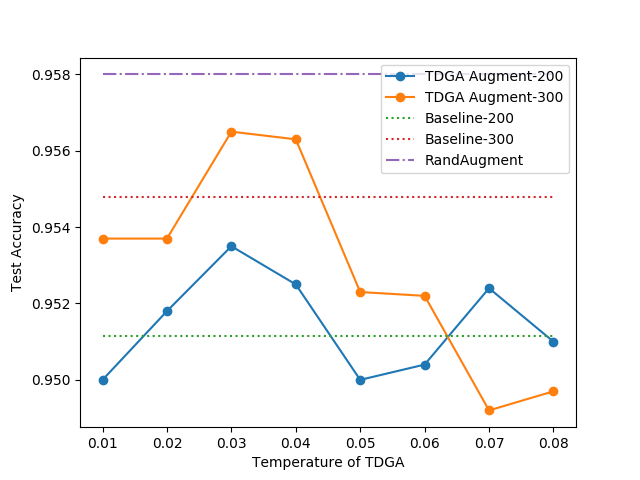
\includegraphics[width=0.7\columnwidth]{exp_change_temperature.png}
      \caption{温度を変化させた Test accuracy(強度固定)}
      \label{fig:exp_change_temperature}
    \end{center}
  \end{figure}

  図 \ref{fig:exp_change_mag} に温度を 0.05 に固定して温度を変化させた Test accuracy を示す.
  \begin{figure}[ht]
    \begin{center}
      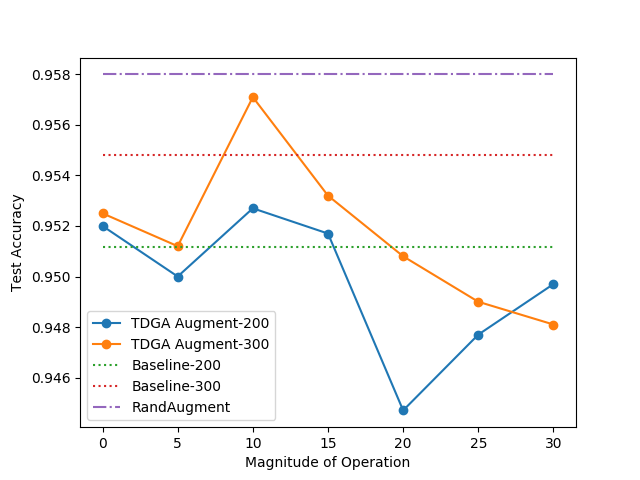
\includegraphics[width=0.7\columnwidth]{exp_change_mag.png}
      \caption{強度を変化させた Test accuracy(温度固定)}
      \label{fig:exp_change_mag}
    \end{center}
  \end{figure}

  エポックを増やすと  accuracy が向上することが確認できた.しかし,baseline からの伸びという点ではそこまでの向上は見られない.得られた拡張も変形を加えないようなものが主であった.この傾向はむしろエポックを増やすほうが顕著に現れそう.

  ここで,図 \ref{fig:transform_importance} に RandAugment で報告されていた,各操作を採用することによる精度向上の表を示す(正確には表ですがスクショしたので図になっています).$\Delta$ はその操作を選択することで最終精度が向上する期待値を表している.

  \begin{figure}[ht]
    \begin{center}
      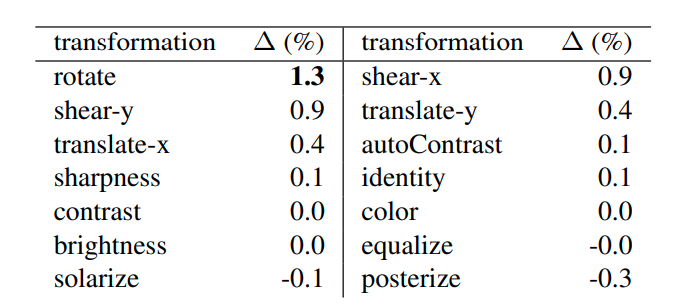
\includegraphics[width=0.7\columnwidth]{operation_importance.png}
      \caption{各操作を選択することによる精度への影響}
      \label{fig:transform_importance}
    \end{center}
  \end{figure}

  これを見るとやはり変形を加えるようなものの方が精度への寄与は大きいことがわかる.このあたりの多様度をどのように維持するのかということが今後の主な課題になりそう.

  表 \ref{tab:compare_cider10} に他手法との比較を示す.比較に用いた手法は Population Based Augmentation (PBA) \cite{DBLP:journals/corr/abs-1905-05393}, Fast AutoAugment (Fast AA) \cite{DBLP:journals/corr/abs-1905-00397}, AutoAugment (AA) \cite{DBLP:journals/corr/abs-1801-02929} および  RandAugment (RA) \cite{Cubuk2019RandAugmentPA} である. TDGA Augment 以外の値は RandAugment で掲載されているものである.また,baseline の値は手元で確認した 200 エポック 10 回試行の平均であり,()内の値は論文で挙げられていたものである.また,Wide-ResNet-28-10 を用いた実験は時間がかかるため(CNN 部分の学習に 200 エポックで 6 時間程度)まずは Wide-ResNet-28-2 でチューニングする.

  \begin{table}[ht]
		\centering
		\caption{Test accuracy(\%) on CIFER-10}
		\label{tab:compare_cider10}
		\begin{tabular}{c||c c c c c|c} \hline
		  &baseline&PBA&Fast AA&AA&RA&TDGA Augment\\ \hline
			Wide-ResNet-28-2&95.10(94.9)&-&-&95.9&95.8&95.35(300epoch:95.71)\\
			Wide-ResNet-28-10&96.32(96.1)&97.4&97.3&97.4&97.3&-\\ \hline
		\end{tabular}
	\end{table}

  \section{RandAugmentの精度が確認できない}
  今使っている CNN モデルに RandAugment を適用したが,論文通りの精度が出ない.CNN 側に問題がないとすれば transform 側にあるので,少し見直してみているところ.RandAugment を PyTorch で実装しているレポでは実際精度が確認できない系の issue が投げられているので,やや怪しいところではある.

	\section{次のタスク}
	操作の種類毎に多様性をもたせるように拡張したい.

  \section{TODO タスク}
  \begin{itemize}{
    \item{個体数,世代数の変化による影響の観察}
    \item{CIFER-100, SVHN,漫画画像など他の画像データセットに対する精度比較}
    \item{他のモデルを用いた実験}
    \item{得られた拡張ポリシーの転移学習および Fine Tuning の可能性の調査}
    \item{検出タスクへの適用}

	}\end{itemize}

	% 参考文献リスト
	\bibliographystyle{unsrt}
	\bibliography{2020_07_31}
\end{document}
